\section{Adjusting the queuing model}\label{sec:scenarios}

With the queuing model established and validated in
Section~\ref{sec:wasserstein}, an investigation into the parameters of the model
can be conducted. This section is comprised of several `what-if' scenarios --- a
classic component of healthcare operational research --- under this novel
parameterisation. The outcomes of interest in this work are server (resource)
utilisation and system times as these capture the both the driving forces of
cost and the overall state of the system. Specifically, the objective of these
experiments is to address the following questions:
\begin{itemize}
    \item How would the system be affected by a change in overall patient
        arrivals?
    \item How is the system affected by a change in resource availability (i.e.\
        a change in \(c\))?
    \item How is the system affected by patients moving between clusters?
\end{itemize}

%TODO Add a disclaimer about relative values here.

\subsection{Changes to overall patient arrivals}\label{subsec:arrivals}

\begin{figure}
    \centering
    \begin{minipage}{\halfimgwidth}
        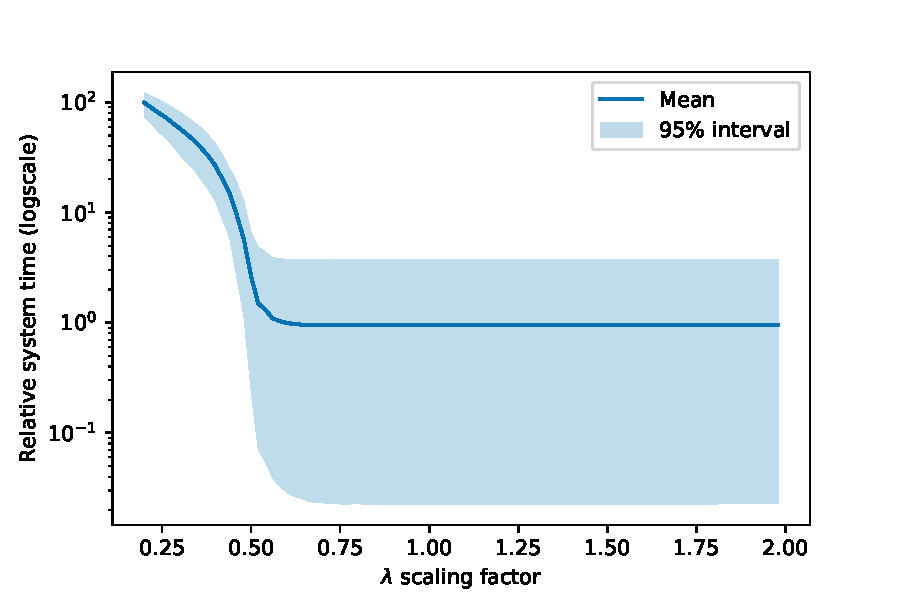
\includegraphics[width=\linewidth]{lambda_time_logscale}
        \captionof{figure}{A plot of \(\lambda\) scaling factor against mean
        relative system time}\label{fig:lambda_time}
    \end{minipage}\hfill%
    \begin{minipage}{\halfimgwidth}
        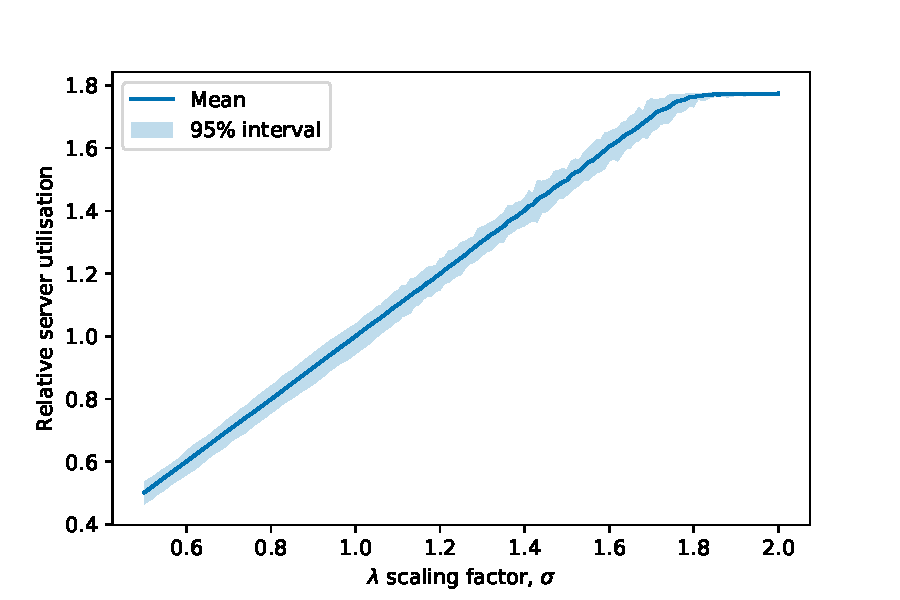
\includegraphics[width=\linewidth]{lambda_utilisation}
        \captionof{figure}{A plot of \(\lambda\) scaling factor against mean
        relative server utilisation}\label{fig:lambda_utilisation}
    \end{minipage}
\end{figure}

\subsection{Changes to resource availability}\label{subsec:resources}

\begin{figure}
    \centering
    \begin{minipage}{\halfimgwidth}
        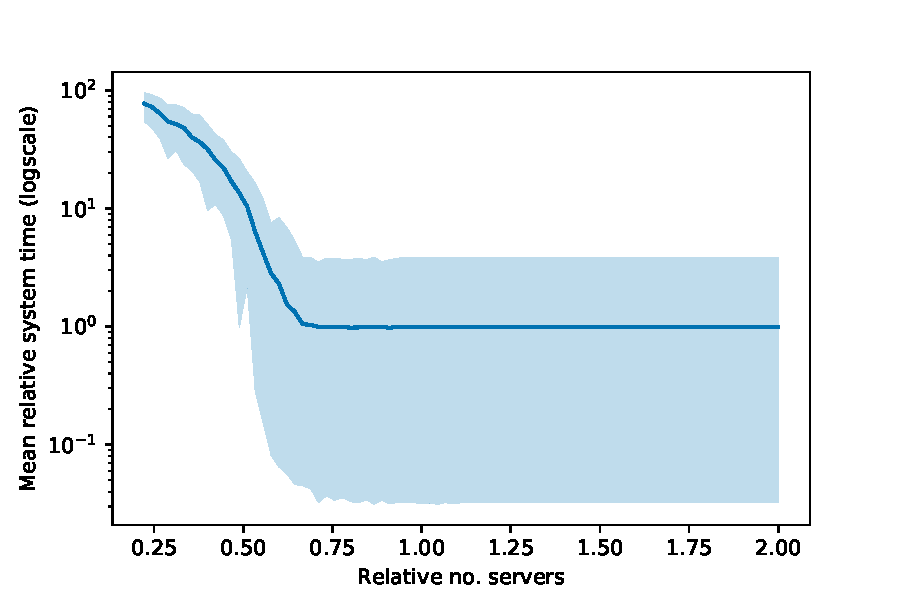
\includegraphics[width=\linewidth]{servers_time_logscale}
        \captionof{figure}{A plot of the number of servers, \(c\), against mean
        relative system time}\label{fig:servers_time}
    \end{minipage}\hfill%
    \begin{minipage}{\halfimgwidth}
        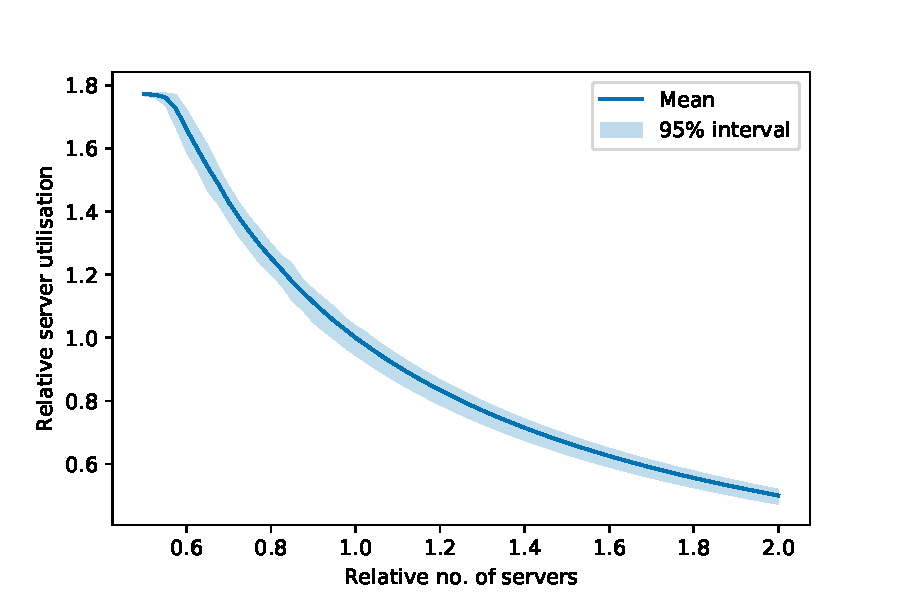
\includegraphics[width=\linewidth]{servers_utilisation}
        \captionof{figure}{A plot of the number of servers, \(c\), against mean
        relative server utilisation}\label{fig:servers_utilisation}
\end{minipage}
\end{figure}

\subsection{Moving patients between clusters}\label{subsec:moving}

\begin{figure}
    \centering
    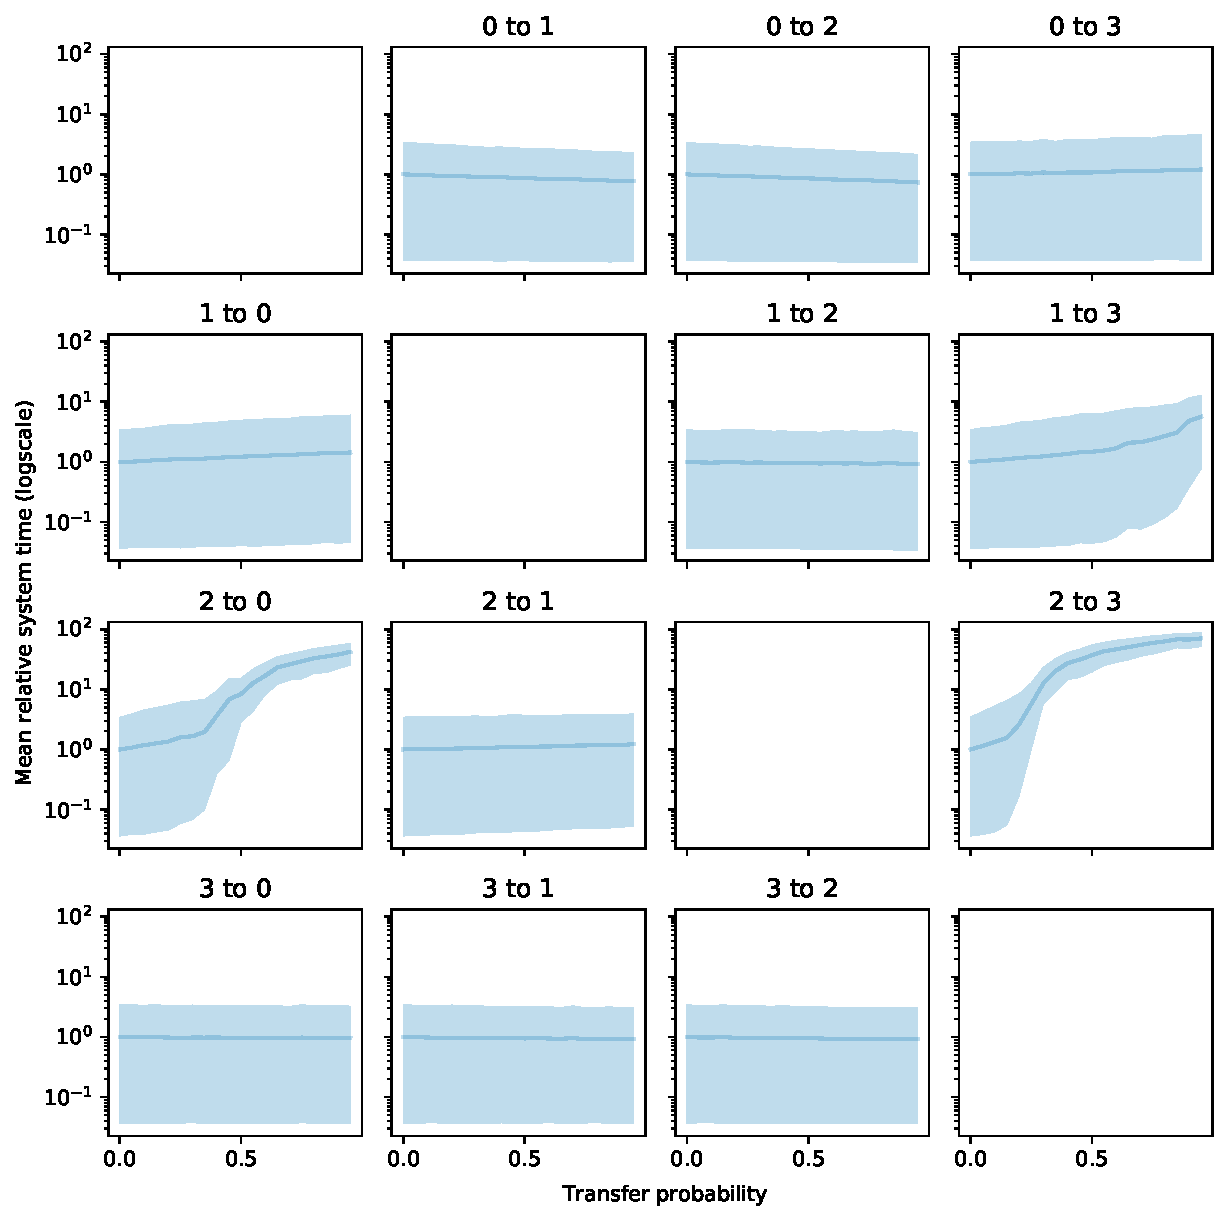
\includegraphics[width=\imgwidth]{moving_time_logscale}
    \caption{Plots showing the effect of proportions of each cluster moving to
    another on the mean relative system time}\label{fig:moving_time}
\end{figure}

\begin{figure}
    \centering
    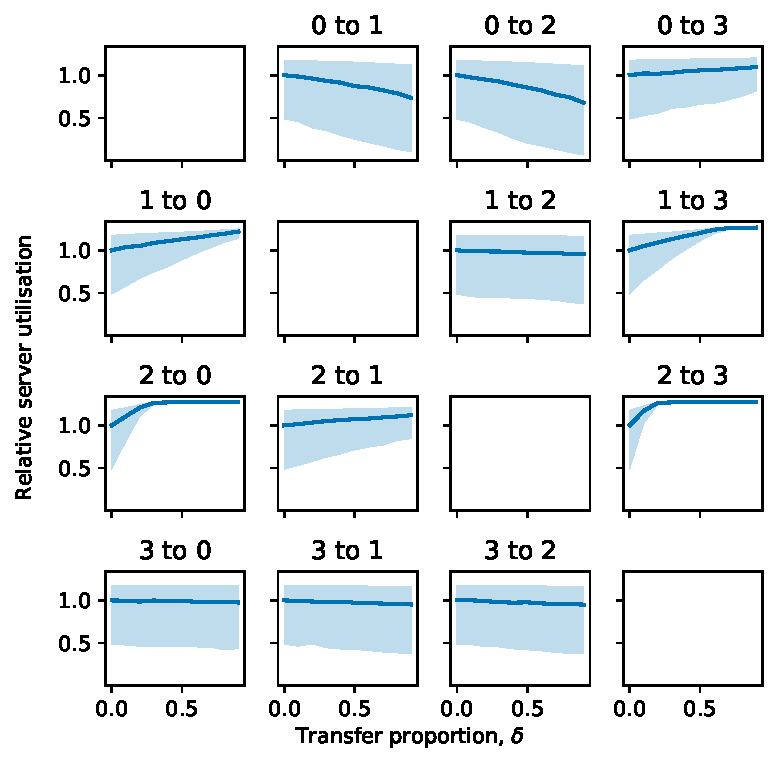
\includegraphics[width=\imgwidth]{moving_utilisation}
    \caption{Plots showing the effect of proportions of each cluster moving to
    another on the mean relative server
    utilisation}\label{fig:moving_utilisation}
\end{figure}
